% Generated by Sphinx.
\def\sphinxdocclass{report}
\documentclass[letterpaper,10pt,english]{sphinxmanual}
\usepackage[utf8]{inputenc}
\DeclareUnicodeCharacter{00A0}{\nobreakspace}
\usepackage{cmap}
\usepackage[T1]{fontenc}
\usepackage{babel}
\usepackage{times}
\usepackage[Bjarne]{fncychap}
\usepackage{longtable}
\usepackage{sphinx}
\usepackage{multirow}


\title{AIMBAT Documentation}
\date{June 09, 2014}
\release{0.1.2}
\author{Lay Kuan Loh, Xiaoting Lou, \& Suzan van der Lee}
\newcommand{\sphinxlogo}{}
\renewcommand{\releasename}{Release}
\makeindex

\makeatletter
\def\PYG@reset{\let\PYG@it=\relax \let\PYG@bf=\relax%
    \let\PYG@ul=\relax \let\PYG@tc=\relax%
    \let\PYG@bc=\relax \let\PYG@ff=\relax}
\def\PYG@tok#1{\csname PYG@tok@#1\endcsname}
\def\PYG@toks#1+{\ifx\relax#1\empty\else%
    \PYG@tok{#1}\expandafter\PYG@toks\fi}
\def\PYG@do#1{\PYG@bc{\PYG@tc{\PYG@ul{%
    \PYG@it{\PYG@bf{\PYG@ff{#1}}}}}}}
\def\PYG#1#2{\PYG@reset\PYG@toks#1+\relax+\PYG@do{#2}}

\expandafter\def\csname PYG@tok@gd\endcsname{\def\PYG@tc##1{\textcolor[rgb]{0.63,0.00,0.00}{##1}}}
\expandafter\def\csname PYG@tok@gu\endcsname{\let\PYG@bf=\textbf\def\PYG@tc##1{\textcolor[rgb]{0.50,0.00,0.50}{##1}}}
\expandafter\def\csname PYG@tok@gt\endcsname{\def\PYG@tc##1{\textcolor[rgb]{0.00,0.27,0.87}{##1}}}
\expandafter\def\csname PYG@tok@gs\endcsname{\let\PYG@bf=\textbf}
\expandafter\def\csname PYG@tok@gr\endcsname{\def\PYG@tc##1{\textcolor[rgb]{1.00,0.00,0.00}{##1}}}
\expandafter\def\csname PYG@tok@cm\endcsname{\let\PYG@it=\textit\def\PYG@tc##1{\textcolor[rgb]{0.25,0.50,0.56}{##1}}}
\expandafter\def\csname PYG@tok@vg\endcsname{\def\PYG@tc##1{\textcolor[rgb]{0.73,0.38,0.84}{##1}}}
\expandafter\def\csname PYG@tok@m\endcsname{\def\PYG@tc##1{\textcolor[rgb]{0.13,0.50,0.31}{##1}}}
\expandafter\def\csname PYG@tok@mh\endcsname{\def\PYG@tc##1{\textcolor[rgb]{0.13,0.50,0.31}{##1}}}
\expandafter\def\csname PYG@tok@cs\endcsname{\def\PYG@tc##1{\textcolor[rgb]{0.25,0.50,0.56}{##1}}\def\PYG@bc##1{\setlength{\fboxsep}{0pt}\colorbox[rgb]{1.00,0.94,0.94}{\strut ##1}}}
\expandafter\def\csname PYG@tok@ge\endcsname{\let\PYG@it=\textit}
\expandafter\def\csname PYG@tok@vc\endcsname{\def\PYG@tc##1{\textcolor[rgb]{0.73,0.38,0.84}{##1}}}
\expandafter\def\csname PYG@tok@il\endcsname{\def\PYG@tc##1{\textcolor[rgb]{0.13,0.50,0.31}{##1}}}
\expandafter\def\csname PYG@tok@go\endcsname{\def\PYG@tc##1{\textcolor[rgb]{0.20,0.20,0.20}{##1}}}
\expandafter\def\csname PYG@tok@cp\endcsname{\def\PYG@tc##1{\textcolor[rgb]{0.00,0.44,0.13}{##1}}}
\expandafter\def\csname PYG@tok@gi\endcsname{\def\PYG@tc##1{\textcolor[rgb]{0.00,0.63,0.00}{##1}}}
\expandafter\def\csname PYG@tok@gh\endcsname{\let\PYG@bf=\textbf\def\PYG@tc##1{\textcolor[rgb]{0.00,0.00,0.50}{##1}}}
\expandafter\def\csname PYG@tok@ni\endcsname{\let\PYG@bf=\textbf\def\PYG@tc##1{\textcolor[rgb]{0.84,0.33,0.22}{##1}}}
\expandafter\def\csname PYG@tok@nl\endcsname{\let\PYG@bf=\textbf\def\PYG@tc##1{\textcolor[rgb]{0.00,0.13,0.44}{##1}}}
\expandafter\def\csname PYG@tok@nn\endcsname{\let\PYG@bf=\textbf\def\PYG@tc##1{\textcolor[rgb]{0.05,0.52,0.71}{##1}}}
\expandafter\def\csname PYG@tok@no\endcsname{\def\PYG@tc##1{\textcolor[rgb]{0.38,0.68,0.84}{##1}}}
\expandafter\def\csname PYG@tok@na\endcsname{\def\PYG@tc##1{\textcolor[rgb]{0.25,0.44,0.63}{##1}}}
\expandafter\def\csname PYG@tok@nb\endcsname{\def\PYG@tc##1{\textcolor[rgb]{0.00,0.44,0.13}{##1}}}
\expandafter\def\csname PYG@tok@nc\endcsname{\let\PYG@bf=\textbf\def\PYG@tc##1{\textcolor[rgb]{0.05,0.52,0.71}{##1}}}
\expandafter\def\csname PYG@tok@nd\endcsname{\let\PYG@bf=\textbf\def\PYG@tc##1{\textcolor[rgb]{0.33,0.33,0.33}{##1}}}
\expandafter\def\csname PYG@tok@ne\endcsname{\def\PYG@tc##1{\textcolor[rgb]{0.00,0.44,0.13}{##1}}}
\expandafter\def\csname PYG@tok@nf\endcsname{\def\PYG@tc##1{\textcolor[rgb]{0.02,0.16,0.49}{##1}}}
\expandafter\def\csname PYG@tok@si\endcsname{\let\PYG@it=\textit\def\PYG@tc##1{\textcolor[rgb]{0.44,0.63,0.82}{##1}}}
\expandafter\def\csname PYG@tok@s2\endcsname{\def\PYG@tc##1{\textcolor[rgb]{0.25,0.44,0.63}{##1}}}
\expandafter\def\csname PYG@tok@vi\endcsname{\def\PYG@tc##1{\textcolor[rgb]{0.73,0.38,0.84}{##1}}}
\expandafter\def\csname PYG@tok@nt\endcsname{\let\PYG@bf=\textbf\def\PYG@tc##1{\textcolor[rgb]{0.02,0.16,0.45}{##1}}}
\expandafter\def\csname PYG@tok@nv\endcsname{\def\PYG@tc##1{\textcolor[rgb]{0.73,0.38,0.84}{##1}}}
\expandafter\def\csname PYG@tok@s1\endcsname{\def\PYG@tc##1{\textcolor[rgb]{0.25,0.44,0.63}{##1}}}
\expandafter\def\csname PYG@tok@gp\endcsname{\let\PYG@bf=\textbf\def\PYG@tc##1{\textcolor[rgb]{0.78,0.36,0.04}{##1}}}
\expandafter\def\csname PYG@tok@sh\endcsname{\def\PYG@tc##1{\textcolor[rgb]{0.25,0.44,0.63}{##1}}}
\expandafter\def\csname PYG@tok@ow\endcsname{\let\PYG@bf=\textbf\def\PYG@tc##1{\textcolor[rgb]{0.00,0.44,0.13}{##1}}}
\expandafter\def\csname PYG@tok@sx\endcsname{\def\PYG@tc##1{\textcolor[rgb]{0.78,0.36,0.04}{##1}}}
\expandafter\def\csname PYG@tok@bp\endcsname{\def\PYG@tc##1{\textcolor[rgb]{0.00,0.44,0.13}{##1}}}
\expandafter\def\csname PYG@tok@c1\endcsname{\let\PYG@it=\textit\def\PYG@tc##1{\textcolor[rgb]{0.25,0.50,0.56}{##1}}}
\expandafter\def\csname PYG@tok@kc\endcsname{\let\PYG@bf=\textbf\def\PYG@tc##1{\textcolor[rgb]{0.00,0.44,0.13}{##1}}}
\expandafter\def\csname PYG@tok@c\endcsname{\let\PYG@it=\textit\def\PYG@tc##1{\textcolor[rgb]{0.25,0.50,0.56}{##1}}}
\expandafter\def\csname PYG@tok@mf\endcsname{\def\PYG@tc##1{\textcolor[rgb]{0.13,0.50,0.31}{##1}}}
\expandafter\def\csname PYG@tok@err\endcsname{\def\PYG@bc##1{\setlength{\fboxsep}{0pt}\fcolorbox[rgb]{1.00,0.00,0.00}{1,1,1}{\strut ##1}}}
\expandafter\def\csname PYG@tok@kd\endcsname{\let\PYG@bf=\textbf\def\PYG@tc##1{\textcolor[rgb]{0.00,0.44,0.13}{##1}}}
\expandafter\def\csname PYG@tok@ss\endcsname{\def\PYG@tc##1{\textcolor[rgb]{0.32,0.47,0.09}{##1}}}
\expandafter\def\csname PYG@tok@sr\endcsname{\def\PYG@tc##1{\textcolor[rgb]{0.14,0.33,0.53}{##1}}}
\expandafter\def\csname PYG@tok@mo\endcsname{\def\PYG@tc##1{\textcolor[rgb]{0.13,0.50,0.31}{##1}}}
\expandafter\def\csname PYG@tok@mi\endcsname{\def\PYG@tc##1{\textcolor[rgb]{0.13,0.50,0.31}{##1}}}
\expandafter\def\csname PYG@tok@kn\endcsname{\let\PYG@bf=\textbf\def\PYG@tc##1{\textcolor[rgb]{0.00,0.44,0.13}{##1}}}
\expandafter\def\csname PYG@tok@o\endcsname{\def\PYG@tc##1{\textcolor[rgb]{0.40,0.40,0.40}{##1}}}
\expandafter\def\csname PYG@tok@kr\endcsname{\let\PYG@bf=\textbf\def\PYG@tc##1{\textcolor[rgb]{0.00,0.44,0.13}{##1}}}
\expandafter\def\csname PYG@tok@s\endcsname{\def\PYG@tc##1{\textcolor[rgb]{0.25,0.44,0.63}{##1}}}
\expandafter\def\csname PYG@tok@kp\endcsname{\def\PYG@tc##1{\textcolor[rgb]{0.00,0.44,0.13}{##1}}}
\expandafter\def\csname PYG@tok@w\endcsname{\def\PYG@tc##1{\textcolor[rgb]{0.73,0.73,0.73}{##1}}}
\expandafter\def\csname PYG@tok@kt\endcsname{\def\PYG@tc##1{\textcolor[rgb]{0.56,0.13,0.00}{##1}}}
\expandafter\def\csname PYG@tok@sc\endcsname{\def\PYG@tc##1{\textcolor[rgb]{0.25,0.44,0.63}{##1}}}
\expandafter\def\csname PYG@tok@sb\endcsname{\def\PYG@tc##1{\textcolor[rgb]{0.25,0.44,0.63}{##1}}}
\expandafter\def\csname PYG@tok@k\endcsname{\let\PYG@bf=\textbf\def\PYG@tc##1{\textcolor[rgb]{0.00,0.44,0.13}{##1}}}
\expandafter\def\csname PYG@tok@se\endcsname{\let\PYG@bf=\textbf\def\PYG@tc##1{\textcolor[rgb]{0.25,0.44,0.63}{##1}}}
\expandafter\def\csname PYG@tok@sd\endcsname{\let\PYG@it=\textit\def\PYG@tc##1{\textcolor[rgb]{0.25,0.44,0.63}{##1}}}

\def\PYGZbs{\char`\\}
\def\PYGZus{\char`\_}
\def\PYGZob{\char`\{}
\def\PYGZcb{\char`\}}
\def\PYGZca{\char`\^}
\def\PYGZam{\char`\&}
\def\PYGZlt{\char`\<}
\def\PYGZgt{\char`\>}
\def\PYGZsh{\char`\#}
\def\PYGZpc{\char`\%}
\def\PYGZdl{\char`\$}
\def\PYGZhy{\char`\-}
\def\PYGZsq{\char`\'}
\def\PYGZdq{\char`\"}
\def\PYGZti{\char`\~}
% for compatibility with earlier versions
\def\PYGZat{@}
\def\PYGZlb{[}
\def\PYGZrb{]}
\makeatother

\begin{document}

\maketitle
\tableofcontents
\phantomsection\label{index::doc}


Contents:


\includegraphics{NU_Logo_purple.jpg}


\chapter{Introduction}
\label{docfiles/introduction:introduction}\label{docfiles/introduction:welcome-to-aimbat-s-documentation}\label{docfiles/introduction::doc}

\section{About AIMBAT}
\label{docfiles/introduction:about-aimbat}
AIMBAT (Automated and Interactive Measurement of Body wave Arrival Times) is an open-source software package for efficiently measuring teleseismic body wave arrival times for large seismic arrays {\hyperref[docfiles/citations:louvanderlee2013]{{[}LouVanDerLee2013{]}}}. It is based on a widely used method called MCCC (Multi-Channel Cross-Correlation) {\hyperref[docfiles/citations:vandecarcrosson1990]{{[}VanDecarCrosson1990{]}}}. The package is automated in the sense of initially aligning seismograms for MCCC which is achieved by an ICCS (Iterative Cross Correlation and Stack) algorithm. Meanwhile, a GUI (graphical user interface) is built to perform seismogram quality control interactively. Therefore, user processing time is reduced while valuable input from a user's expertise is retained. As a byproduct, SAC {\hyperref[docfiles/citations:goldsteindodge2003]{{[}GoldsteinDodge2003{]}}} plotting and phase picking functionalities are replicated and enhanced.

Modules and scripts included in the AIMBAT package were developed using \href{http://www.python.org/}{Python programming language} and its open-source modules on the Mac OS X platform since 2009. The original MCCC {\hyperref[docfiles/citations:vandecarcrosson1990]{{[}VanDecarCrosson1990{]}}} code was transcribed into Python. The GUI of AIMBAT was inspired and initiated at the \href{http://www.iris.edu/hq/es\_course/content/2009.html}{2009 EarthScope USArray Data Processing and Analysis Short Course}. AIMBAT runs on Mac OS X, Linux/Unix and Windows thanks to the platform-independent feature of Python. It has been tested on Mac OS 10.6.8 and 10.7 and Fedora 16.

The AIMBAT software package is distributed under the \href{http://www.gnu.org/licenses/gpl.html}{GNU General Public License Version 3 (GPLv3)} as published by the Free Software Foundation.


\section{Associated Documents}
\label{docfiles/introduction:associated-documents}\begin{itemize}
\item {} 
\code{Seismological Research Letters Paper}

\item {} 
\code{PDF Version of Manual}. Automatically generated from these online docs, please excuse minor issues that may arise from automated conversion.

\end{itemize}


\section{Authors' Contacts}
\label{docfiles/introduction:authors-contacts}\label{docfiles/introduction:id5}\begin{itemize}
\item {} 
\href{http://lkloh2410.wordpress.com/}{Lay Kuan Loh}

Email: \href{mailto:lkloh@cmu.edu}{lkloh@cmu.edu}

\item {} 
\href{http://www.earth.northwestern.edu/~xlou/Welcome.html}{Xiaoting Lou}

Email: \href{mailto:xlou@u.northwestern.edu}{xlou@u.northwestern.edu}

\item {} 
\href{http://www.earth.northwestern.edu/research/suzan/}{Suzan van der Lee}

Email: \href{mailto:suzan@earth.northwestern.edu}{suzan@earth.northwestern.edu}

\end{itemize}


\chapter{Installing Python Dependencies}
\label{docfiles/install_dependencies::doc}\label{docfiles/install_dependencies:installing-python-dependencies}
Usually, Macs already have python installed by default. To check if you have python on your mac, open up terminal, and do python in the terminal. If python is installed you should see a python console show up, displaying the version number of python. The version number should be at least 2.7 or higher. If python is not installed, you should see an error message show up. However, you may or may not have some necessary packages installed.


\section{Getting Git}
\label{docfiles/install_dependencies:getting-git}
The \href{https://github.com/pysmo}{latest version of AIMBAT} will be on Github, so it would be good to get \href{https://github.com/}{Git} on your computer. This is not strictly necessary, as you could also download it as a zipfile from the \emph{AIMBAT website \textless{}http://www.earth.northwestern.edu/\textasciitilde{}xlou/aimbat.html\textgreater{}\_}.

The best way to get Git is to use \href{https://mac.github.com/}{Git for Mac}. This is a GUI you can used for your repositories, but if you want to use the command line interface you can also enable it when setting it up.


\section{Getting your operating system}
\label{docfiles/install_dependencies:getting-your-operating-system}
We assume that most users of AIMBAT will be using macs. If our assumptions are wrong, please {\hyperref[docfiles/introduction:authors-contacts]{\emph{contact the authors}}}, and if there is sufficient interest we will construct documentation for installations on other operating systems as well.

On a mac, to find the version of your operating system, first click on the apple icon on the top bar of your desktop, go to \code{System Preferences}, and click on \code{Startup Disk}. The operating system version should then be displayed.

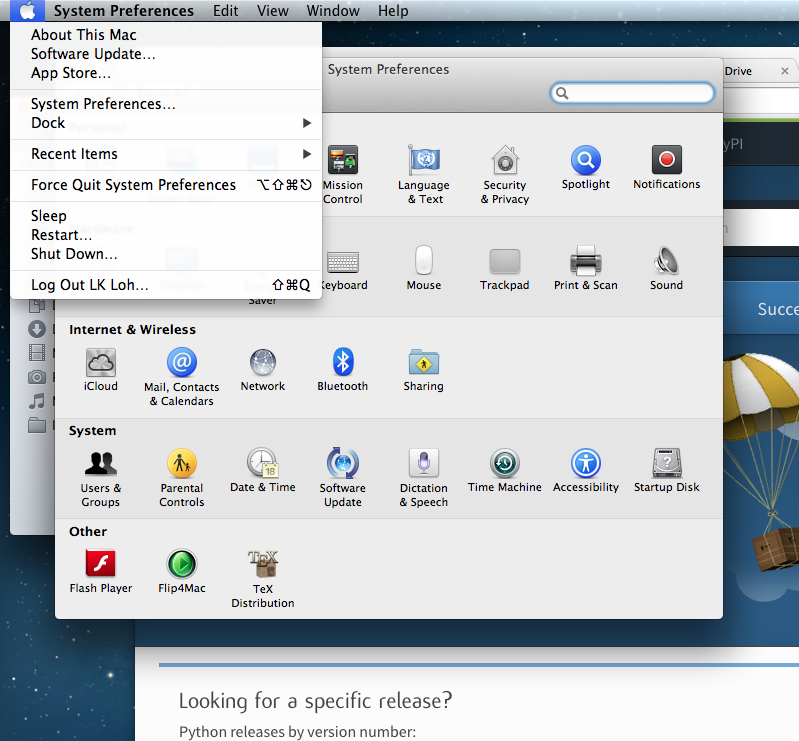
\includegraphics{system_preferences.png}


\section{Python Packages needed}
\label{docfiles/install_dependencies:python-packages-needed}
The following are required for AIMBAT
* \href{http://www.numpy.org/}{Numpy}
* \href{http://www.scipy.org/}{Scipy}
* \href{http://matplotlib.org/}{Matplotlib}

Using \href{http://ipython.org/}{iPython} is optional but recommended, as iPython is an interactive console designed to make


\section{Installing Python with Enthought Canopy}
\label{docfiles/install_dependencies:installing-python-with-enthought-canopy}
\href{http://www1.i2r.a-star.edu.sg/~lins/codes/python.html}{Shaowei Lin} suggested \href{https://www.enthought.com/store/}{Enthought Canopy} to install all the Python packages easily. If you download the free version of Express Enthought Canopy, it gives you everything you need for installing AIMBAT properly.

If you do not want to use Enthought Canopy, read the rest of this section.


\section{Installing Python with Macports}
\label{docfiles/install_dependencies:installing-python-with-macports}

\section{Possible Issues}
\label{docfiles/install_dependencies:possible-issues}
Here some common problems and possible resolutions. If your problem is not listed here, or you have a suggestion, please {\hyperref[docfiles/introduction:authors-contacts]{\emph{contact the authors}}}.


\subsection{Macport}
\label{docfiles/install_dependencies:macport}
You may run into problems with AIMBAT if your \href{http://www.macports.org/}{Macport} version is not compatible with your operating system version. For example, if you used Macports for OS X 10.8 to install AIMBAT, then upgraded your operating system or OS X 10.9, you may find that AIMBAT no longer works properly. You will need to upgrade Macports to fix this error.

Do not uninstall MacPorts unless you know what you are doing, uninstalling MacPorts may get rid of other programs you installed using MacPorts. However, if you are sure you want to do so, see \href{https://guide.macports.org/chunked/installing.macports.uninstalling.html}{here} for instructions.


\subsection{Installing Python with Pip}
\label{docfiles/install_dependencies:installing-python-with-pip}
Be careful with the operating system. For OS X 10.9 and above, Python 2.7 is not fully compatible and there may be problems installing python with Pip. Best to use Enthought Canopy or Python 3 with OS X 10.9.


\subsection{Setting the Python Path to the scripts}
\label{docfiles/install_dependencies:setting-the-python-path-to-the-scripts}
You are asked to add the path to the AIMBAT scripts in your file. To do that, you add them to the \code{.bashrc} file. There are other files you could add it to that work as well, such as the \code{.profile} or \code{.bash\_profile} files. You can see the files by opening the terminal and doing \code{ls -a} to see all the hidden files, and open then by doing \code{vi .bashrc} in vim, for instance.
To ensure you can open a script, you need to add:

\begin{Verbatim}[commandchars=\\\{\}]
export PATH=\PYGZdl{}PATH:\PYGZlt{}path\PYGZhy{}to\PYGZhy{}folder\PYGZhy{}with\PYGZhy{}scripts\PYGZgt{}
export PYTHONPATH=\PYGZdl{}PYTHONPATH:\PYGZlt{}path\PYGZhy{}to\PYGZhy{}folder\PYGZhy{}with\PYGZhy{}scripts\PYGZgt{}
\end{Verbatim}

to the \code{.bashrc} file. We recommend adding the paths to the \code{.bashrc} file.


\subsection{Terminal Commands stop working}
\label{docfiles/install_dependencies:terminal-commands-stop-working}
If ever the terminal commands such as ls stop working in the terminal, it could be that something went wrong with a path in the \code{.bashrc} or \code{.profile} files. If that happens you may not be able to open them in vim as that command would have stopped working as well. Instead, in the terminal, you do:

\begin{Verbatim}[commandchars=\\\{\}]
PATH=/bin:\PYGZdl{}\PYGZob{}PATH\PYGZcb{}
PATH=/usr/bin:\PYGZdl{}\PYGZob{}PATH\PYGZcb{}
\end{Verbatim}

And that should allow the commands to start working again. Figure out what you did wrong and remove that command.


\subsection{Installing Enthought Canopy}
\label{docfiles/install_dependencies:installing-enthought-canopy}
Occasionally, Enthought Canopy may not open the default setup environment after you downloaded and tried to install it. If this happens, open the Canopy package, go to ``Preferences'', and select Canopy as your default environment.

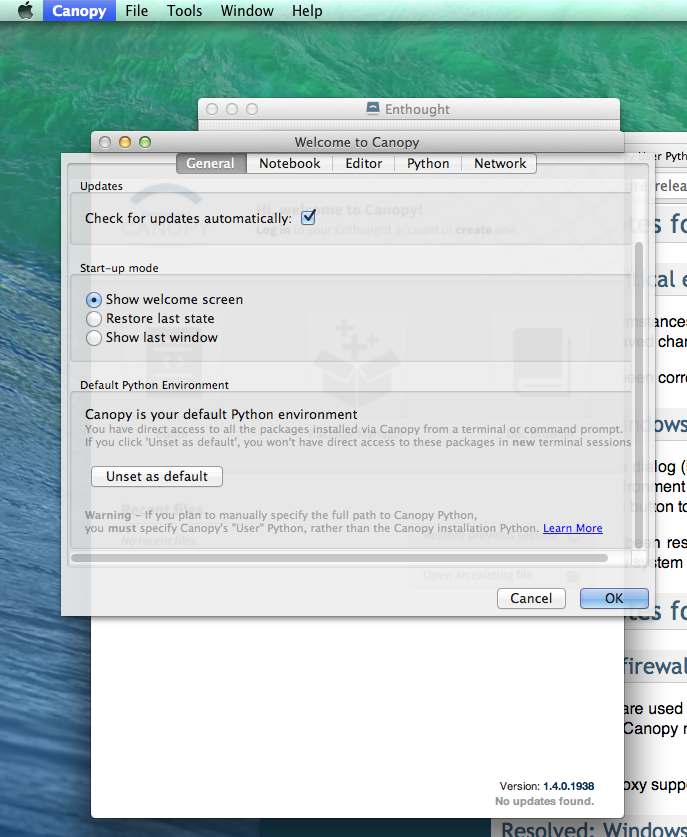
\includegraphics{enthought_as_default.png}


\subsection{Uninstalling Enthought Canopy}
\label{docfiles/install_dependencies:uninstalling-enthought-canopy}
The official Enthought gives suggestions on uninstalling \href{https://guide.macports.org/chunked/installing.macports.uninstalling.html}{here}.

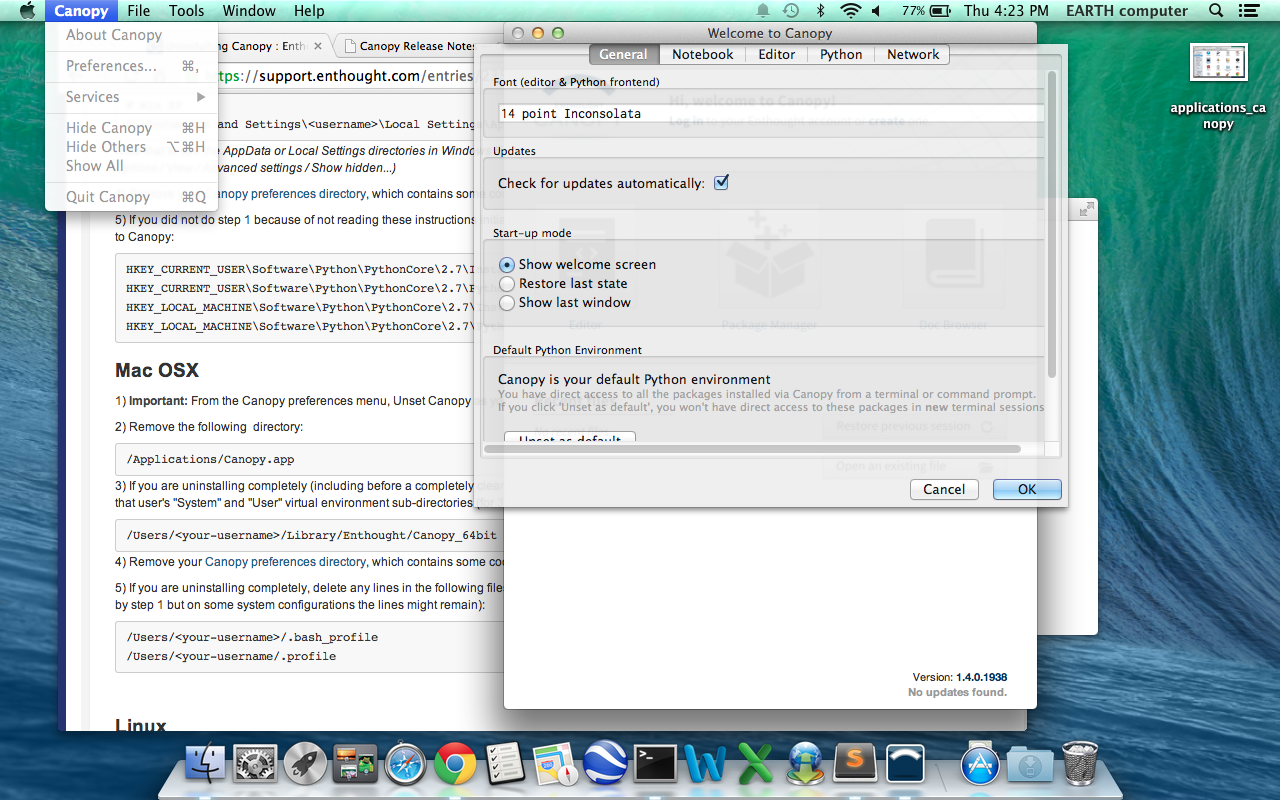
\includegraphics{canopy_preferences.png}

STEPS:
\begin{enumerate}
\item {} 
From the Canopy preferences menu, unset Canopy as your default Python.

\item {} 
For each Canopy user, delete the following directory which contains that user’s ``System'' and ``User'' virtual environment subdirections.

\item {} 
Delete Canopy from the Applications folder.

\item {} 
Clean up the hidden files. Delete anything referencing Canopy or Enthought in the hidden files, as evidence by referencing \code{ls -a} in your home directory. Check the \code{.bashrc} and \code{.profile} directories first. If Enthought is not completely gone, this happens if you call Python.

\item {} 
(Optional). Keep doing \code{which python} and cleaning the python files that show up, until \code{which python} gives you nothing when you type it in the terminal.

\end{enumerate}

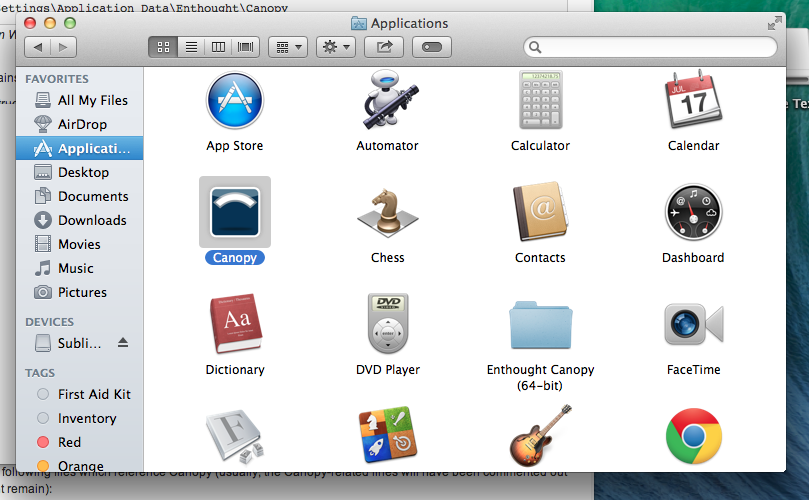
\includegraphics{applications_canopy.png}


\subsection{Path to python files not found}
\label{docfiles/install_dependencies:path-to-python-files-not-found}
After adding the path to your directory with scripts in \code{.bashrc}, you still need to source the \code{.bashrc} files in \code{.profile}, or the system may not find the directory. See here for more \href{http://publib.boulder.ibm.com/infocenter/pseries/v5r3/index.jsp?topic=/com.ibm.aix.baseadmn/doc/baseadmndita/prof\_file.htm}{details} to see how the profile file is sourced. Note that this one will override the file in \emph{/etc/profile}.

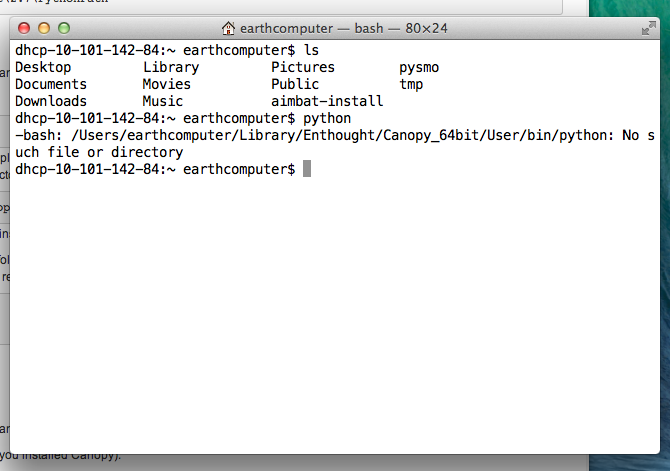
\includegraphics{residue.png}

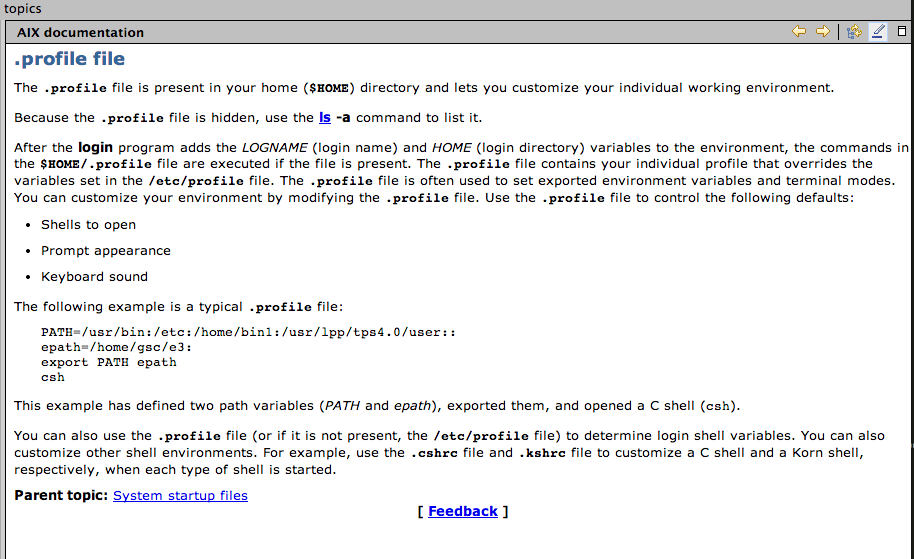
\includegraphics{profile_file.png}

\href{http://linux.die.net/man/1/bash}{This explanation} explains how the bashrc file is sourced.

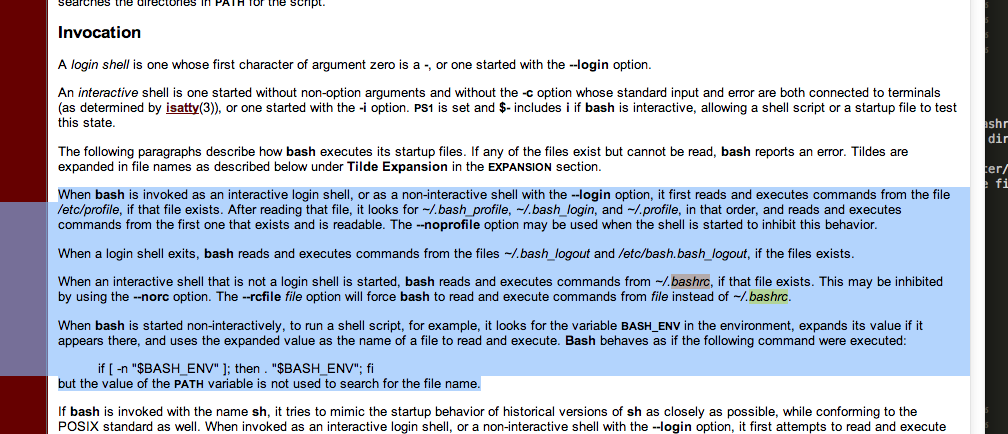
\includegraphics{bashrc_file.png}

This is what the bashrc and profile files should look like on your home directory:

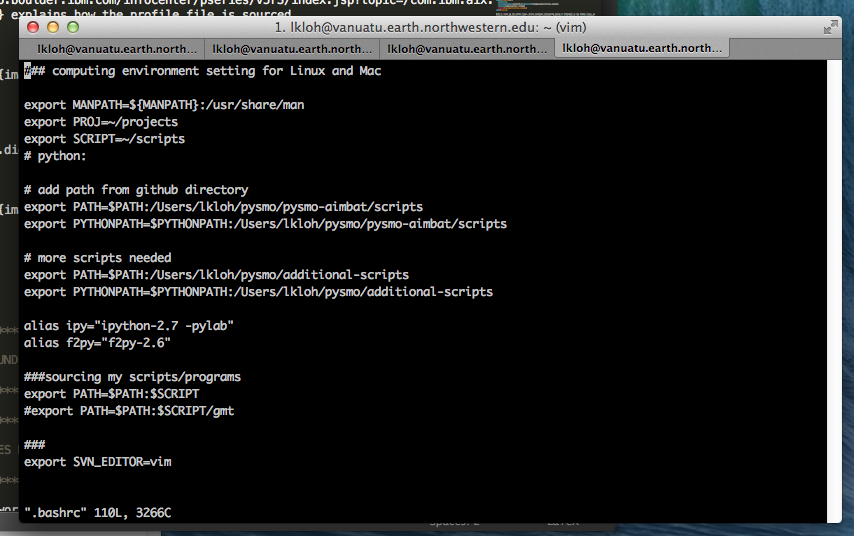
\includegraphics{bashrc_home.png}

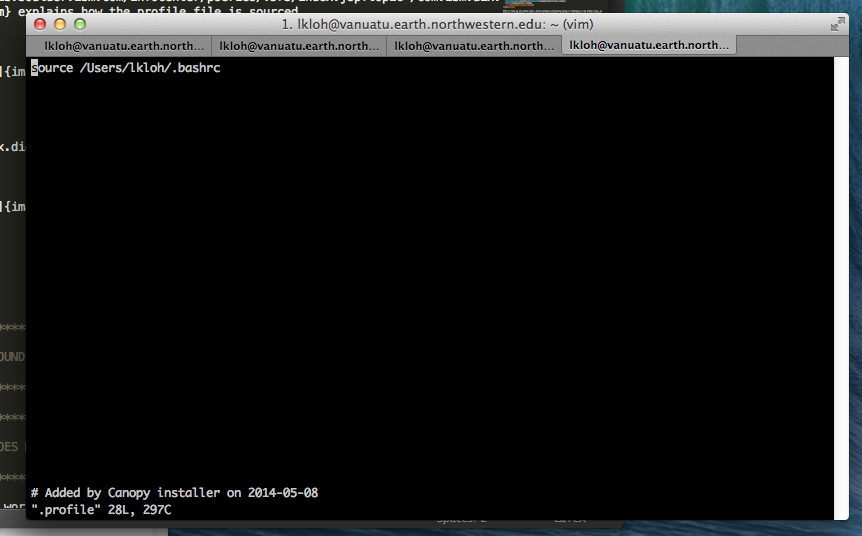
\includegraphics{profile_home.png}


\chapter{Installing AIMBAT}
\label{docfiles/install_aimbat::doc}\label{docfiles/install_aimbat:installing-aimbat}

\section{Getting the Packages}
\label{docfiles/install_aimbat:getting-the-packages}
AIMBAT is released as a sub-package of pysmo in the name of \code{pysmo.aimbat} along with another sub-package \code{pysmo.sac}. The latest stable release of AIMBAT is available for download at the \href{http://www.earth.northwestern.edu/~xlou/aimbat.html}{official project webpage}.

We are working on a new release of AIMBAT, available on \href{https://github.com/pysmo}{Github}. We are adding more features to make using AIMBAT more convenient, and fixing some bugs in the old code. Download \href{https://github.com/pysmo/aimbat}{pysmo.aimbat} and \href{https://github.com/pysmo/sac}{pysmo.sac} from Github. You will now have two folders called \code{aimbat} and \code{sac} respectively.


\section{Where to install the packages}
\label{docfiles/install_aimbat:where-to-install-the-packages}
There are several options to install the packages. If you just want to use AIMBAT, it is best to store it somewhere where you would not touch the packages so easily, such as the Python \code{site-packages} directory. If you would like to make some changes to the Python code, it is best to store it somewhere pretty accessible, such as your \code{home} directory on your computer, or in \code{Documents}.


\subsection{Installing into the Python Site-Packages Directory}
\label{docfiles/install_aimbat:installing-into-the-python-site-packages-directory}
To find out where the Python Site-Packages Directory is, in the python console, do:

\begin{Verbatim}[commandchars=\\\{\}]
\PYG{k+kn}{import} \PYG{n+nn}{site}\PYG{p}{;}
\PYG{n}{site}\PYG{o}{.}\PYG{n}{getsitepackages}\PYG{p}{(}\PYG{p}{)}
\end{Verbatim}

Whatever is output is obtained, lets call it \code{\textless{}pkg-install-dir\textgreater{}}. Make a directory called \code{pysmo}, and place the sac and aimbat directories inside \code{\textless{}pkg-install-dir\textgreater{}/pysmo}.


\subsection{Installing into the home directory}
\label{docfiles/install_aimbat:installing-into-the-home-directory}
Open your terminal. Type \code{open .} and that will open your home directory. Transfer the \code{aimbat} and \code{sac} repositories inside there.


\section{Building the Pysmo Packages}
\label{docfiles/install_aimbat:building-the-pysmo-packages}
You need to be an administrator on the computer you are installing AIMBAT in, as you need to run the commands with \code{sudo}.


\subsection{Building pysmo.sac}
\label{docfiles/install_aimbat:building-pysmo-sac}
Python module \code{Distutils} is used to write a setup.py script to build, distribute, and install \code{pysmo.sac}. cd into the \code{sac} directory on the command line and run:

\begin{Verbatim}[commandchars=\\\{\}]
sudo python setup.py build
sudo python setup.py install
\end{Verbatim}

If you successfully installed the sac module, in the python console, this should happen after you type \code{from pysmo import sac}


\subsection{Installing pysmo.aimbat}
\label{docfiles/install_aimbat:installing-pysmo-aimbat}
Three sub-directories are included in the \code{aimbat} directory
* \code{example}: Example SAC files
* \code{scripts}: Python scripts to run at the command line
* \code{src}: Python modules to install

The core cross-correlation functions are written in both Python/Numpy (\code{xcorr.py}) and Fortran (\code{xcorr.f90}). Therefore, we need to use Numpy’s \code{Distutils} module for enhanced support of Fortran extension. The usage is similar to the standard Disutils.

Note that some sort of Fortran compiler must already be installed first. Specify them in place of gfortran in the following commands.

cd into the directory the \code{aimbat} package was placed in, and type:

\begin{Verbatim}[commandchars=\\\{\}]
sudo python setup.py build \PYGZhy{}\PYGZhy{}fcompiler=gfortran
sudo python setup.py install
\end{Verbatim}

to install the \code{src} directory.

Add \code{\textless{}path-to-folder\textgreater{}/aimbat/scripts} to environment variable \code{PATH} in a shells start-up file for command line execution of the scripts.
\begin{description}
\item[{Bash Shell Users:}] \leavevmode
\code{export PATH=\$PATH:\textless{}path-to-folder\textgreater{}/aimbat/scripts} in \code{.bashrc} files.

\item[{C Shell Users:}] \leavevmode
\code{setenv PATH=\$PATH:\textless{}path-to-folder\textgreater{}/aimbat/scripts} in \code{.bashrc} files.

\end{description}

If AIMBAT has beenn installed, type from \code{pysmo import aimbat} in a Python shell, and no errors should appear.


\chapter{Getting Data}
\label{docfiles/gettingData:getting-data}\label{docfiles/gettingData::doc}
There are several ways to obtain data to input to AIMBAT. If want to suggest other tools, please {\hyperref[docfiles/introduction:authors-contacts]{\emph{contact the authors}}}.


\section{Standing Order for Data}
\label{docfiles/gettingData:standing-order-for-data}
From the \href{http://www.seis.sc.edu/index.html}{SOD} website:
\begin{quote}

Standing Order for Data, is a framework to define rules to select seismic events, stations, and data. It then allows you to apply processing to the events, stations, and data and currently contains a large set of rules that allow you to select with great precision in these items. The processes mainly consist of simple data transformation and retrieval, but SOD defines hooks to allow you to cleanly insert your own processing steps, either written in Java or an external program.
\end{quote}


\subsection{Installing SOD}
\label{docfiles/gettingData:installing-sod}
First, download \href{http://www.seis.sc.edu/index.html}{SOD}.

Once you have gotten the folder for SOD, put it somewhere where you won't touch it too much. What I did was put the SOD folder in my home directory, though other places are acceptable as well, as long as its not too easy to delete it by accident.

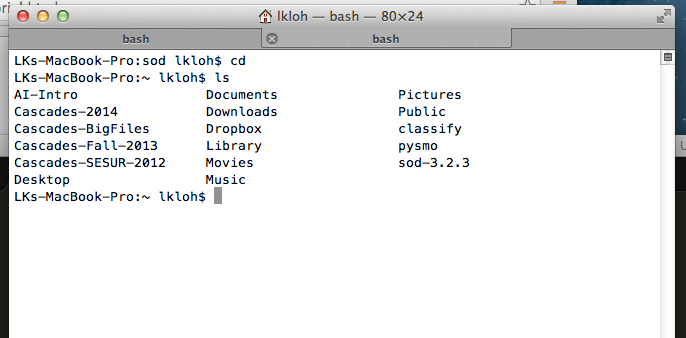
\includegraphics{sod_location.png}

Once you have it there, get the path to the sod folder's bin and put it in your path folder.

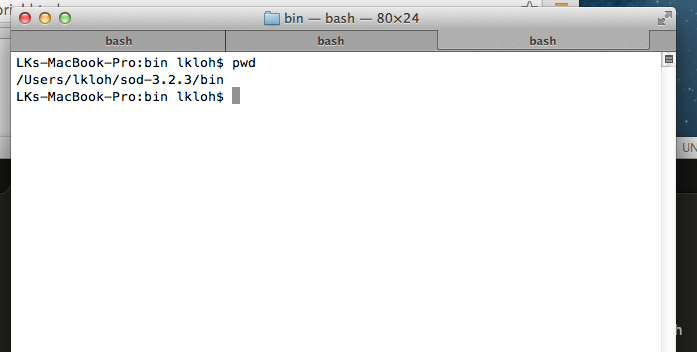
\includegraphics{path_to_sod_bin.png}

Inside my home directory's bash profile (you get the by typing \emph{cd}), you put the path to \emph{sod-3.2.3/bin} by adding in either the \emph{bash} or \emph{bash\_profile} or \emph{profile} files:


\subsection{Downloading Data with SOD}
\label{docfiles/gettingData:downloading-data-with-sod}\begin{quote}\begin{description}
\item[{Authors}] \leavevmode
\href{http://www.earth.northwestern.edu/~trevor/Welcome.html}{Trevor Bollmann}

\end{description}\end{quote}
\begin{enumerate}
\item {} \begin{description}
\item[{Create a sod recipe and place it in the folder that you would like the data to download to.}] \leavevmode\begin{itemize}
\item {} 
\code{sod -f \textless{}recipename\textgreater{}.xml}

\end{itemize}

\end{description}

\item {} \begin{description}
\item[{Run \code{sodcut.sh} to cut the seismogram around phase wanted}] \leavevmode\begin{itemize}
\item {} 
check model within \code{cutevseis.sh}

\item {} 
run using \code{sodcut.sh \textless{}name\textgreater{}}

\item {} 
watch \code{sdir = processed seismograms}

\item {} 
Run over the entire downloaded directory (the files sod downloaded)

\end{itemize}

\end{description}

\item {} \begin{description}
\item[{Run \code{sodpkl.sh} (converts \emph{.sac} files to python pickles)}] \leavevmode\begin{itemize}
\item {} 
run using \code{sodpkl.sh {[}options{]} \textless{}directory\textgreater{}}

\item {} 
output will automatically be zipped

\item {} 
run in DATA directory

\end{itemize}

\end{description}

\item {} \begin{description}
\item[{Run \code{ttpick.py} (does travel time picking with plotting)}] \leavevmode\begin{itemize}
\item {} 
can use \code{iccs.py} but it does not have plotting capabilities

\item {} 
run using \code{ttpick.py {[}options{]} \textless{}pkl.gz file\textgreater{}}

\item {} 
do this one event at a time

\item {} 
use \code{sacp2} to look at the stacking of the seismograms

\item {} 
you can sort the seismograms using the \code{–s} flag

\end{itemize}

\end{description}

\item {} \begin{description}
\item[{run \code{getsta.py} (creates a \code{loc.sta} file)}] \leavevmode\begin{itemize}
\item {} 
\code{getsta.py {[}options{]} \textless{}pkl.gz files\textgreater{}}

\end{itemize}

\end{description}

\item {} \begin{description}
\item[{Run EITHER of these:}] \leavevmode\begin{itemize}
\item {} 
FIRST CHOICE

\end{itemize}

run \code{mccc2delay.py} (converts mccc delays to actual delays) by doing \code{mccc2delay.py {[}option{]} \textless{}.mcp files\textgreater{}}

run \code{getdelay.py} (creates a delay file) by doing \emph{getdelay.py {[}options{]} \textless{}*.px\textgreater{}}. Can possibly use \emph{doplotsta.sh}, plots all of the events and their station delays

Run \code{evmcdelay.sh}
\begin{itemize}
\item {} 
SECOND CHOICE

\end{itemize}

\code{ttcheck.py} to compare the delay times of the p and s waves. Should form a nice cloud with the mean value in line with the cloud.

\end{description}

\item {} \begin{description}
\item[{If you need to remove a station from an event you can use \code{pklsel.py}}] \leavevmode\begin{itemize}
\item {} 
Run using \code{pklsel.py {[}pkl file{]} –d {[}stnm{]}} to remove one station

\item {} 
Only works for one event at a time

\end{itemize}

\end{description}

\item {} \begin{description}
\item[{If you need to filter the data to be able to pick use \code{evsacbp.sh}}] \leavevmode\begin{itemize}
\item {} 
run using \code{evsacbp.sh {[}pkl file{]} bp1 bp2}

\item {} 
Automatically uses two corners

\item {} 
run in the whole downloaded directory (the one with the sac directory)

\end{itemize}

\end{description}

\end{enumerate}


\chapter{Analyzing Data}
\label{docfiles/analyzingData:analyzing-data}\label{docfiles/analyzingData::doc}

\section{Seismic Analysis Code (SAC)}
\label{docfiles/analyzingData:seismic-analysis-code-sac}
AIMBAT uses \href{http://www.iris.edu/files/sac-manual/}{Seismic Analysis Code (SAC)} formatting for some of the files it runs and outputs. To get SAC, you will need to fill out a software request form available on the IRIS website.


\chapter{Parameter Configuration}
\label{docfiles/parameterConfiguration:parameter-configuration}\label{docfiles/parameterConfiguration::doc}

\section{Backend}
\label{docfiles/parameterConfiguration:backend}
\href{http://matplotlib.org/contents.html}{Matplotlib} works with six GUI (Graphical User Interface) toolkits:
\#. WX
\#. Tk
\#. Qt(4)
\#. FTK
\#. Fltk
\#. macosx

The GUI of AIMBAT uses the following to support interactive plotting:
\#. \href{http://matplotlib.org/api/widgets\_api.html}{GUI neutral widgets}
\#. \href{http://matplotlib.org/users/event\_handling.html}{GUI neutral event handling API (Application Programming Interface)}

Examples given in this documentation are using the default toolkit \code{Tk} and backend \code{TkAgg}.

Visit these pages for an \href{http://matplotlib.org/faq/usage\_faq.html\#what-is-a-backend}{explanation of the backend} and \emph{how to customize it \textless{}http://matplotlib.org/users/customizing.html\#customizing-matplotlib\textgreater{}}.

\textbf{Put the following line in you {}`{}`matplotlibrc{}`{}` file:}:

\begin{Verbatim}[commandchars=\\\{\}]
backend : TkAgg \PYGZsh{}Agg rendering to a Tk canvas
\end{Verbatim}

Other parameters for the package can be set up by a configuration file \code{ttdefaults.conf}, which is interpreted by the module ConfigParser. This configuration file is searched in the following order:
\begin{enumerate}
\item {} 
file \code{ttdefaults.conf} in the current working directory

\item {} 
file \code{.aimbat/ttdefaults.conf} in your \code{HOME} directory

\item {} 
a file specified by environment variable \code{TTCONFIG}

\item {} 
file \code{ttdefaults.conf} in the directory where AIMBAT is installed

\end{enumerate}

Python scripts in the \code{\textless{}pkg-install-dir\textgreater{}/pysmo-aimbat-0.1.2/scripts} can be executed from the command line. The command line arguments are parsed by the optparse module to improve the scripts' exibility. If conflicts existed, the command line options override the default parameters given in the configuration file \code{ttdefaults.conf}. Run the scripts with the \code{-h} option for the usage messages.


\chapter{Measuring Teleseismic Body Wave Arrival Times}
\label{docfiles/PickingTravelTimes::doc}\label{docfiles/PickingTravelTimes:measuring-teleseismic-body-wave-arrival-times}
The core idea in using AIMBAT to measure teleseismic body wave arrival times has two parts:
\begin{itemize}
\item {} 
automated phase alignment, to reduce user processing time, and

\item {} 
interactive quality control, to retain valuable user inputs.

\end{itemize}


\section{Automated Phase Alignment}
\label{docfiles/PickingTravelTimes:automated-phase-alignment}
The ICCS algorithm calculates an array stack from predicted time picks, cross-correlates each seismogram with the array stack to Find the time lags at maximum cross-correlation, then use the new time picks to update the array stack in an iterative process. The MCCC algorithm cross-correlates each possible pair of seismograms and uses a least-squares method to calculate an optimized set of relative arrival times. Our method is to combine ICCS and MCCC in a four-step procedure using four anchoring time picks \(_0T_i,\,_1T_i,\,_2T_i,\) and \(_3T_i\).
\begin{enumerate}
\item {} 
Coarse alignment by ICCS

\item {} 
Pick phase arrival at the array stack

\item {} 
Refined alignment by ICCS

\item {} 
Final alignment by MCCC

\end{enumerate}

The one-time manual phase picking at the array stack in step (b) allows the measurement of absolute arrival times. The detailed methodology and procedure can be found in {\hyperref[docfiles/citations:louvanderlee2013]{{[}LouVanDerLee2013{]}}}.


\begin{threeparttable}
\capstart\caption{Time picks and their SAC headers used in the procedure for measuring teleseismic body wave arrival times.}

\begin{tabular}{|p{0.136\linewidth}|p{0.136\linewidth}|p{0.136\linewidth}|p{0.136\linewidth}|p{0.136\linewidth}|p{0.136\linewidth}|p{0.136\linewidth}|}
\hline
 \multirow{2}{*}{
Step
} &  \multirow{2}{*}{
Algorithm
} &  \multicolumn{3}{l|}{
Input
} &  \multicolumn{2}{l|}{
Output
}\\
 & 
Time Window
 &  & 
Time Pick
 & 
Time Header
 & 
Time Pick
 & 
Time Header
\\
\begin{enumerate}
\item {} 
\end{enumerate}
 & 
ICCS
 & 
\(W_a\)
 & 
\(_0T_i\)
 & 
\textbf{T0}
 & 
\(_1T_i\)
 & 
\textbf{T1}
\\
\begin{enumerate}
\setcounter{enumi}{1}
\item {} 
\end{enumerate}
 & 
ICCS
 & 
\(W_b\)
 & 
\(_2T'_i\)
 & 
\textbf{T2}
 & 
\(_2T_i\)
 & 
\textbf{T2}
\\
\begin{enumerate}
\setcounter{enumi}{3}
\item {} 
\end{enumerate}
 & 
MCCS
 & 
\(W_b\)
 & 
\(_2T_i\)
 & 
\textbf{T2}
 & 
\(_3T_i\)
 & 
\textbf{T3}
\\
\hline\end{tabular}

\end{threeparttable}


The ICCS and MCCC algorithms are implemented in two modules \code{pysmo.aimbat.algiccs} and \code{pysmo.aimbat.algmccc}, and can be executed in scripts \code{iccs.py} and \code{mccc.py} respectively.


\section{Picking Travel Times}
\label{docfiles/PickingTravelTimes:picking-travel-times}
This section explains how to run the program \code{ttpick.py} to get the travel times you want.


\subsection{Getting into the right directory}
\label{docfiles/PickingTravelTimes:getting-into-the-right-directory}
In the terminal, cd into the directory with all the \code{pkl} files you want to run. You want to run either the \code{.bht} or \code{.bhz} files. \code{bht} files are for S-waves and bhz files are for P-waves. \code{PKL} is a bundle of \code{SAC} files. Each \code{SAC} file is a seismogram, but since you there may be many seismograms from various stations for each event, we bundle them into a \code{PKL} file so we only have to import one file into AIMBAT, not a few hundred of them.


\subsection{Running ttpick.py}
\label{docfiles/PickingTravelTimes:running-ttpick-py}
Run \code{ttpick/py \textless{}path-to-pkl-file\textgreater{}}. A GUI should pop up if you successfully ran it. Note that if you click on the buttons, they will not work until you move the mouse off them; this is a problem we are hoping to fix.

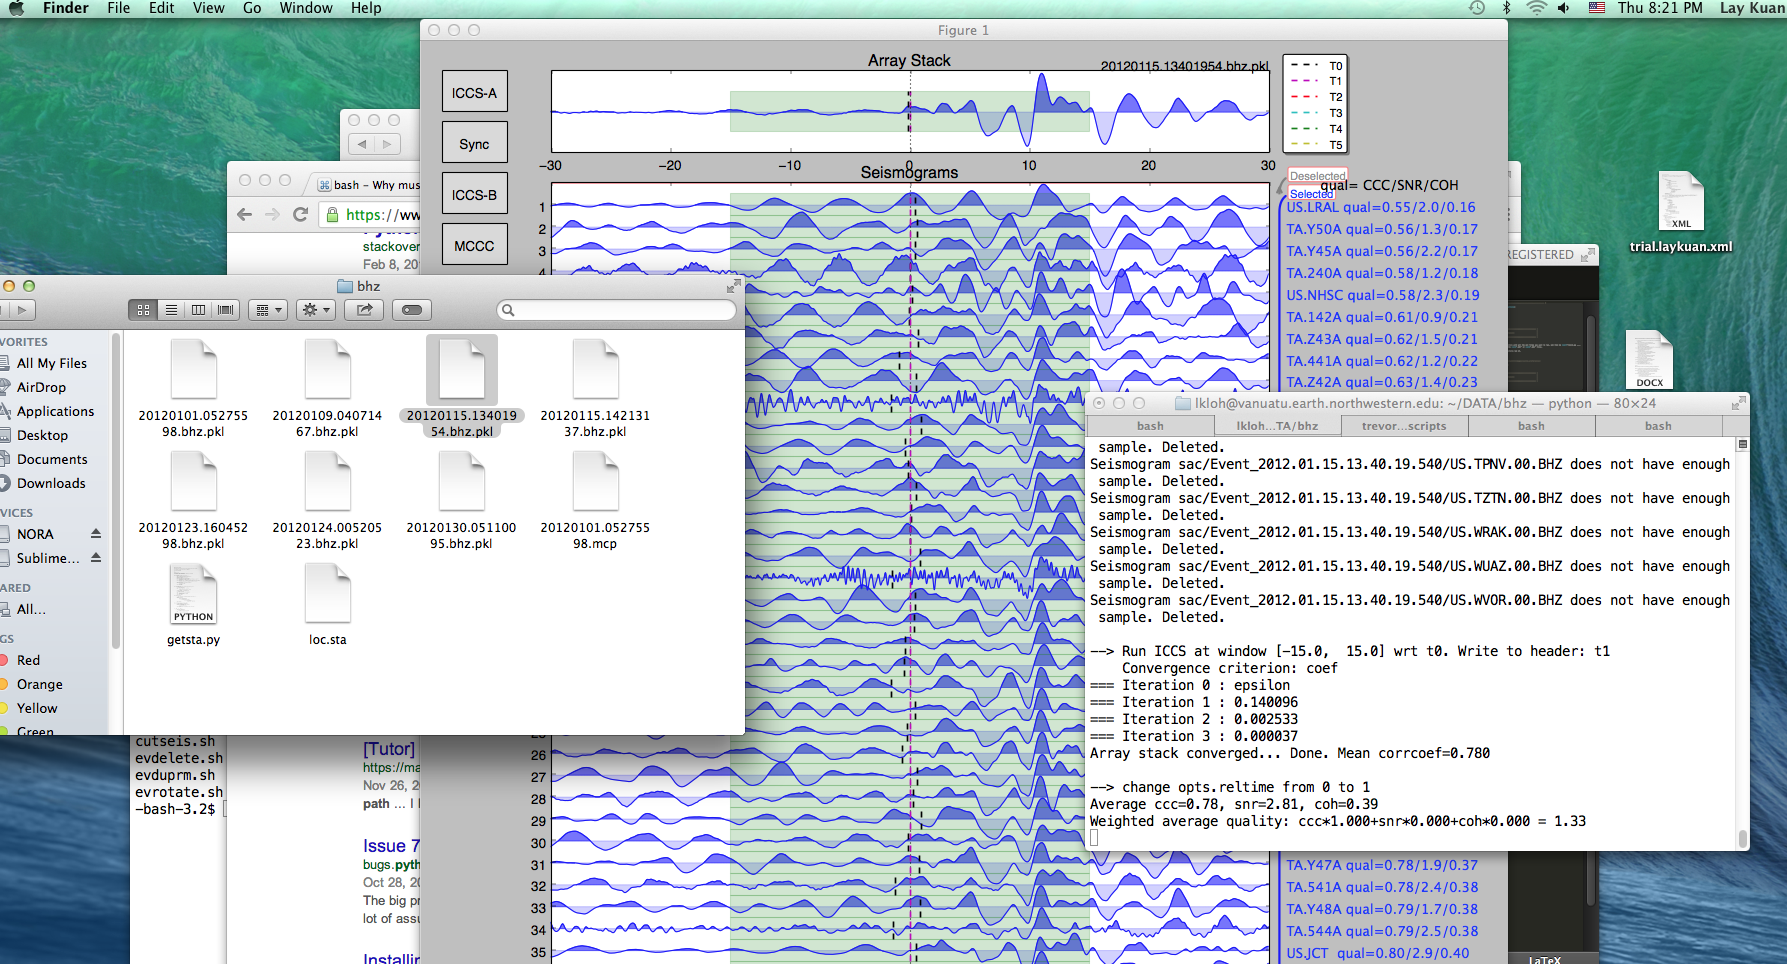
\includegraphics{pick_travel_times.png}


\subsection{ICCC-A}
\label{docfiles/PickingTravelTimes:iccc-a}
\code{ICCC-A} is only used in the beginning, if you have altered some of the travel time arrivals of the seismograms by pressing \code{t2}, and want to realign the array stack.


\subsection{Get rid of really bad seismograms}
\label{docfiles/PickingTravelTimes:get-rid-of-really-bad-seismograms}
If there are any really bad seismograms, you can click on them to deselect them. Bad seismograms are those that look nothing like the shape of the array stack pictured. Usually, if there are more than enough seismograms, so it is safe to throw out any that deviate more than a bit from the array stack.


\subsection{Filtering}
\label{docfiles/PickingTravelTimes:filtering}
To filter your data, hit the \code{filter} button, and a window will popup for you to use the \href{http://en.wikipedia.org/wiki/Butterworth\_filter}{Butterworth filter} to filter your data.

Remember to save your work periodically once you start picking your travel times, otherwise if AIMBAT crashes, you lose it.

You can choose the order by selecting one of the values provided (default is 1), and choose the low and high frequencies for bandpassing by clicking on the appropriate start and stop frequency on the lower graph.


\subsection{ICCC-B}
\label{docfiles/PickingTravelTimes:iccc-b}
Hit the \code{ICCC-B} button to begin the initial cross-correlations. These appear as red lines.

We are not using \code{ICCC-A} here, but these are the theoretical arrival times, marked in black.


\subsection{MCCC}
\label{docfiles/PickingTravelTimes:mccc}
Hit \code{MCCC} to run the Multi-Channel cross-correlation. Do not hit \code{ICCC-A} or \code{ICCC-B} again, or all your work will be erased. A warning will pop up to check if you really do want to hit these two buttons if you do click on them.


\subsection{Manually pick the arrival times using t2}
\label{docfiles/PickingTravelTimes:manually-pick-the-arrival-times-using-t2}
For an earthquake, it is expected that the arrival times should be identical in an idealize situation. However, since stations are located in 3D space, this is not necessarily the case. For earthquakes of magnitude 7.0 and above, usually the arrival times are very well aligned as the signal is high. However, if the earthquake is too strong, the source gets complicated, so it needs filtering.

Below a magnitude of 6.0, the signal to noise ratio gets very weak. If the weighted average quality gets too low (1.0 and below), it may not be worth keeping that data set unless you really need it.

We manually pick the the arrival times to align them. Click on the GUI window, hover over the correct spot where you want to pick the new travel time, and type \code{t2}. A red line should appear exactly where your mouse was. You can zoom in to help you with this picking. To zoom out, just hit \code{MCCC} again.

Also pick the arrival time on the array stack. For the arrival times, you want to align the point where the first peak occurs most of all, then try to get the peaks to align.


\subsection{SACP2 to check for outlier seismograms}
\label{docfiles/PickingTravelTimes:sacp2-to-check-for-outlier-seismograms}
Hit and go to the last figure, (d). Zoom in to have a better look. Zooming in doesn’t always work well; close and reopen the \code{SACP2} window if there are problems.

Click on the outliers that stray from the main group of stacked seismograms. The terminal will output the names of the seismograms that you clicked on, so you can return to the main GUI window and readjust the travel times.


\subsection{Go through the badly aligned seismograms and realign the travel times manually}
\label{docfiles/PickingTravelTimes:go-through-the-badly-aligned-seismograms-and-realign-the-travel-times-manually}
By default, the worst seismograms are on the first page, and as you click through the pages, the quality of the seismograms gradually gets better. Keep using \code{t2} to realign the arrival times so that the peaks of all the seismograms are nicely aligned. Remember to zoom in to have a better look.

However, you may which to sort the seismograms in alphabetical order so that you can find the bad seismogrrams and correct them more easily. Hit the \code{sort} button and a window will popup for you to choose which sorting method to use. In this case, choose to sort the files by filename.

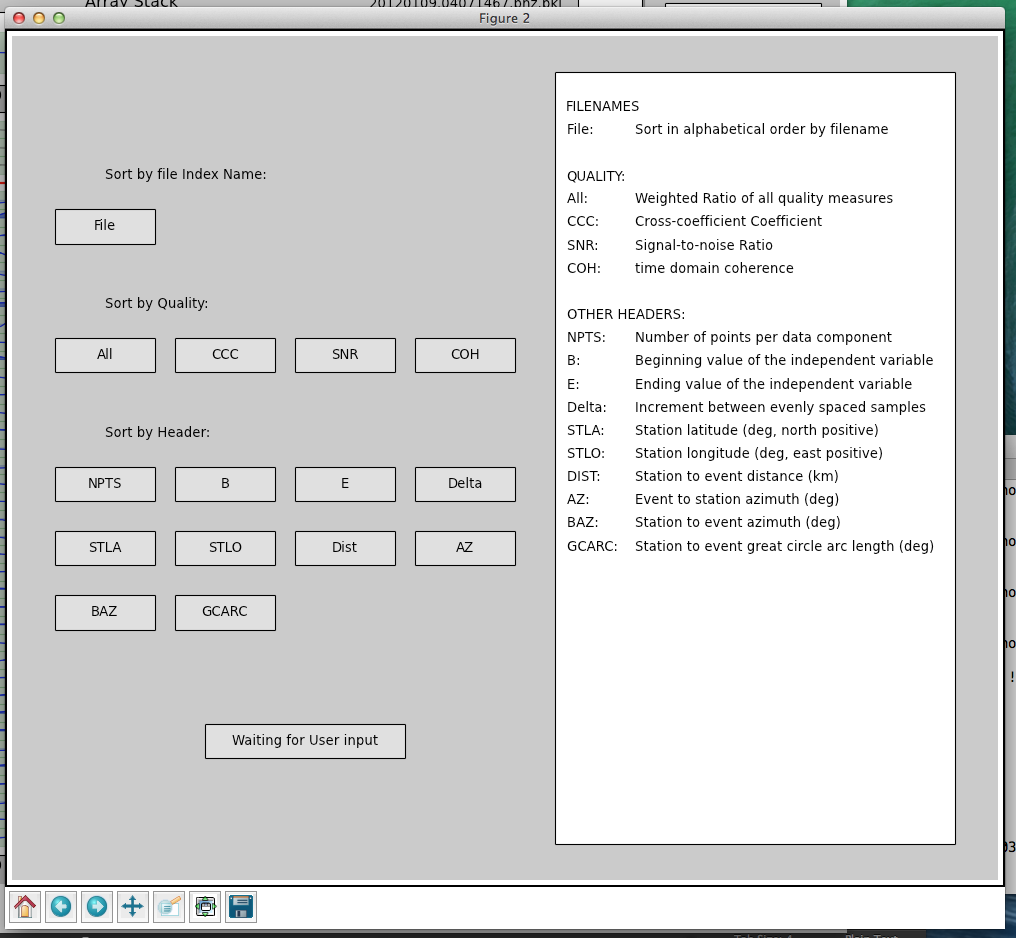
\includegraphics{sorting-interface.png}

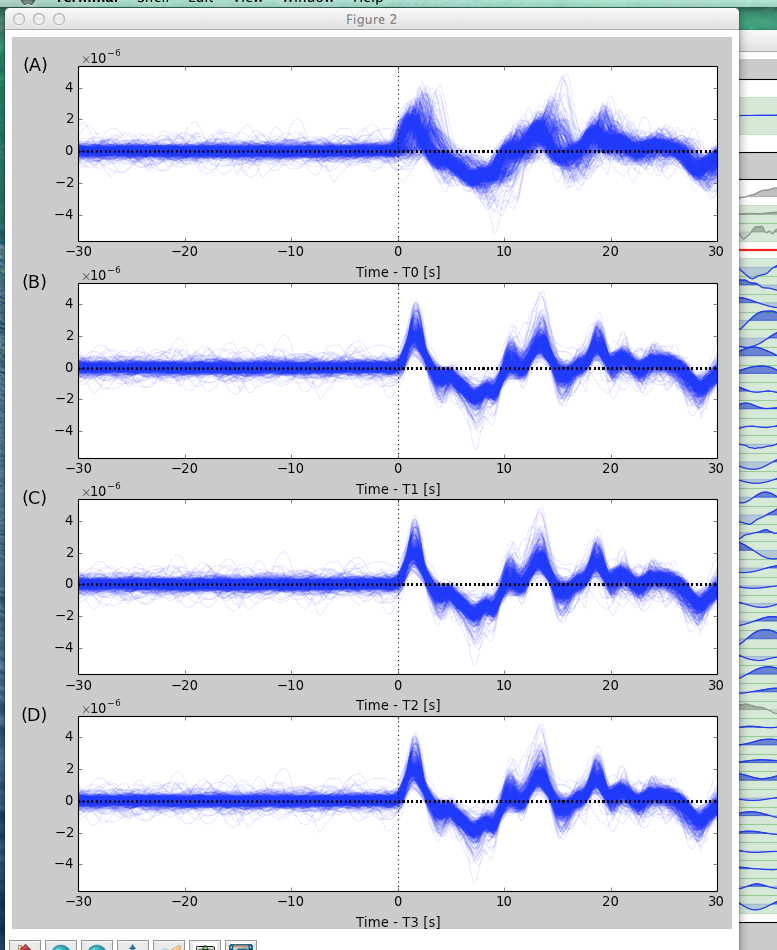
\includegraphics{SACP2_popup.png}

The seismograms are stretched to fit together, but they may be scaled differently.


\section{What the Alignments Stand For}
\label{docfiles/PickingTravelTimes:what-the-alignments-stand-for}\begin{itemize}
\item {} 
T0: Theoretical Arrival

\item {} 
T1: Pick from initial cross correlation

\item {} 
T2: Travel Time pick

\item {} 
T3: MCCC pick

\item {} 
T4: Zoom in

\end{itemize}


\section{Post Processing}
\label{docfiles/PickingTravelTimes:post-processing}

\subsection{Getting the output}
\label{docfiles/PickingTravelTimes:getting-the-output}
In the same folder as the initial PKL file you ran \code{ttpick.py} on, you can find the output list with extension \code{\textless{}event name\textgreater{}.mcp}, which contains the travel time arrivals.


\subsection{Getting the stations of the seismograms chosen}
\label{docfiles/PickingTravelTimes:getting-the-stations-of-the-seismograms-chosen}
Run \code{getsta.py} in the additional scripts (not on Github for now). It gives the unique list of stations where the seismograms came from. You need to run it with the list of all \code{pkl} files chosen after you saved to. You so this \code{./getsta.py *.pkl}.

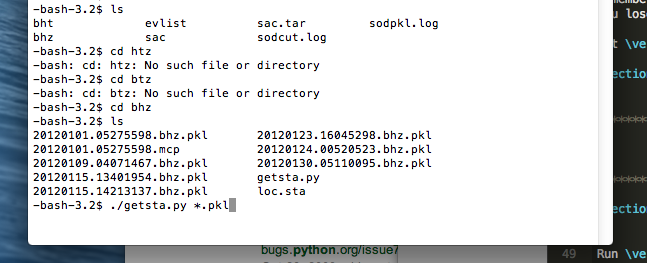
\includegraphics{count_stations.png}


\subsection{Picking Travel Times does not work}
\label{docfiles/PickingTravelTimes:picking-travel-times-does-not-work}
If you run \code{ttick.py \textless{}Event name\textgreater{}.bhz.pkl}, a GUI will pop up for you to manually pick the travel times by pressing the keyboard. If typing on the keyboard as directed does not allow you to pick travel times, it could be a problem with the keyboard settings, or the matplotlib backend.

To fix this, first look for the .matplotlib directory. It is hidden so in your home directory do \code{ls -a} to find it.
Once you have found the \code{.matplotlib} directory, cd into it, and then look for the \code{matplotlibrc} file.
Inside that file, ensure the backend is set to:

\begin{Verbatim}[commandchars=\\\{\}]
backend : TkAgg
\end{Verbatim}

Comment out the other backends!


\subsection{Travel Times}
\label{docfiles/PickingTravelTimes:travel-times}
If one of the seismograms being picked does not fit completely within the green (computer) window, nad you hit \emph{ICCC-A} or \emph{ICCC-B}, you will get an error message complaining about the exact seismogram which is too short. Deselect it.


\chapter{Citations}
\label{docfiles/citations:citations}\label{docfiles/citations::doc}

\chapter{Indices and tables}
\label{index:indices-and-tables}\begin{itemize}
\item {} 
\emph{genindex}

\item {} 
\emph{modindex}

\item {} 
\emph{search}

\end{itemize}

\begin{thebibliography}{VanDecarCrosson1990}
\bibitem[GoldsteinDodge2003]{GoldsteinDodge2003}{\phantomsection\label{docfiles/citations:goldsteindodge2003} 
Goldstein, P., D. Dodge, M. Firpo, and L. Minner (2003), SAC2000: Signal processing and analysis tools for seismologists and engineers, International Geophysics, 81, 1613–1614.
}
\bibitem[Hunder2007]{Hunder2007}{\phantomsection\label{docfiles/citations:hunder2007} 
Hunter, J. (2007), Matplotlib: A 2D Graphics Environment, Computing in Science \& Engineering, 3(9), 90–95.
}
\bibitem[LouVanDerLee2013]{LouVanDerLee2013}{\phantomsection\label{docfiles/citations:louvanderlee2013} 
AIMBAT: A Python/Matplotlib Tool for Measuring Teleseismic Arrival Times. Xiaoting Lou, Suzan van der Lee, and Simon Lloyd (2013), Seismol. Res. Lett., 84(1), 85-93, doi:10.1785/0220120033.
}
\bibitem[VanDecarCrosson1990]{VanDecarCrosson1990}{\phantomsection\label{docfiles/citations:vandecarcrosson1990} 
VanDecar, J. C., and R. S. Crosson (1990), Determination of teleseismic relative phase arrival times using multi-channel cross-correlation and least squares, Bulletin of the Seismological Society of America, 80(1), 150–169.
}
\end{thebibliography}



\renewcommand{\indexname}{Index}
\printindex
\end{document}
